\section{Experimental Results}

\subsection{Experimental Settings}
We use our curated cardiac arrest cohort from CHOA-CICU to conduct 5-fold cross-validation. We further ensure that no patient appears in both the training and testing sets for an unbiased evaluation.
As defined in Sec.~\ref{sec:study}, our research problem, early risk prediction of CA, is formulated asa a binary classification task. Accordingly, we employ a broad set of binary classification metrics, including balanced accuracy (Bal\_Acc), F1 score, Matthews Correlation Coefficient (MCC), Area Under the Precision-Recall Curve (AUPRC), and Area Under the Receiver Operating Characteristic Curve (AUROC), to comprehensively assess model performance while accounting for the inherent class imbalance (admission-wise CA incidence $=3.1\%$). 
% talk about the metrics a bit
In our evaluation, CA events are treated as the positive class. 
Among these metrics, Bal\_Acc is a specifically designed metric to avoid inflated performance on imbalanced dataset, which is essentially arithmetic mean of sensitivity and specificity in binary classification case. F1 is a harmonic mean of the precision and recall. 
MCC is defined as
\begin{equation}
    \text{MCC}=\frac{tp\times tn - fp \times fn}{\sqrt{(tp+fp)(tp+fn)(tn+fp)(tn+fn)}},
\end{equation}
where is generally regarded as a balanced metric for imbalanced case. A MCC of $+1$ presents a perfect prediction, $0$ an random prediction, and $-1$ an inverse prediction. AUROC and AUPRC both assess trade-offs between key performance rates. While AUROC is widely used—providing a threshold-independent evaluation of the balance between TPR and FPR and serving as a valuable benchmark for comparison with prior work—AUPRC is often more informative in scenarios with class imbalance~\cite{tomavsev2021use}, as it emphasizes the trade-off between precision and recall and focuses on performance for the minority (positive) class.

\begin{table*}[ht!]
\centering
\centering
\caption{Experimental results on CHOA-CICU curated cohort (numbers in percentage).}
\label{tab:CHOA_main_exp}
\begin{tabular}{c|ccccc}
\toprule
Model & Bal\_Acc & F1 & MCC & AUPRC &AUROC\\
\multicolumn{6}{c}{\textit{Clinician Derived Risk Scores}} \\
KNN-Dtw &  $51.65 \pm 3.71$ & $2.06 \pm 4.61$ & $1.36 \pm 3.35$ & $3.81 \pm 0.91$ & $55.27 \pm 4.21$ \\
SVC-Gak &  $50.00 \pm 0.00$ & $0.00 \pm 0.00$ & $0.00 \pm 0.00$ & $6.19 \pm 2.21$ & $54.72 \pm 3.80$\\
\midrule
\multicolumn{6}{c}{\textit{Last Observed Risk Factors}} \\
KNN-Unif &  $50.22 \pm 0.72$ & $1.18 \pm 2.63$ & $1.83 \pm 5.62$ & $4.53 \pm 1.24$ & $57.41 \pm 2.99$\\
LR &  $49.80 \pm 0.77$ & $2.70 \pm 1.56$ & $-0.39 \pm 1.52$ & $4.60 \pm 0.49$ & $62.92 \pm 1.92$\\
RF-Gini &  $50.00 \pm 0.00$ & $0.00 \pm 0.00$ & $0.00 \pm 0.00$ & $7.05 \pm 0.81$ & $73.29 \pm 2.47$ \\
XGBoost & $\underline{61.03} \pm 3.18$ & $\underline{11.80} \pm 1.96$ & $\underline{10.18} \pm 2.45$ & $6.88 \pm 1.18$ & $72.35 \pm 4.00$ \\
LightGBM &  $53.74 \pm 5.28$ & $8.62 \pm 5.92$ & $5.24 \pm 6.96$ & $5.82 \pm 2.26$ & $61.42 \pm 11.06$\\
TabNN &  $50.84 \pm 0.64$ & $3.90 \pm 2.33$ & $1.82 \pm 1.68$ & $5.34 \pm 0.79$ & $62.16 \pm 3.64$\\
\hline
\multicolumn{6}{c}{\textit{Numerical Time-Series Risk Factors}} \\
TResNet & $53.93 \pm 2.80$ & $10.32 \pm 4.54$ & $7.47 \pm 4.83$ & $7.53 \pm 1.95$ & $72.21 \pm 7.22$\\
gMLP & $52.51 \pm 1.64$ & $8.05 \pm 3.54$ & $5.11 \pm 3.54$ & $\underline{8.72} \pm 3.13$ & $\textbf{75.04} \pm 3.52$ \\
\hline
\multicolumn{6}{c}{\textbf{\textit{Our Proposed Tabular-Textual Multimodal Risk Factors}}} \\
\modelname & $\mathbf{63.08}\pm 3.65$ & $\mathbf{14.31}\pm 2.28$ & $\mathbf{13.18}\pm 2.55$ & $\textbf{9.15} \pm 3.16$ & $\underline{73.99} \pm 3.16$\\
\bottomrule
\end{tabular}
\vspace{-0.3cm}
\end{table*}

\subsection{Compared Baseline Models}
To comprehensively evaluate the effectiveness of our proposed model, we include ten other AI models. As we summarize before that the EHR data used for pediatric CA is heterogeneous and multi-resolution, the ten AI models can be categories into the following three groups with different EHR feature processing techniques.
\subsubsection{Clinician Derived Risk Scores} We use Pediatric Early Warning Score (PEWS)~\cite{monaghan2005pews} to process EHR data, which involves assessing a range of vital signs and clinical observations—such as heart rate, respiratory rate, blood pressure, oxygen saturation, and behavioral changes—assigning scores based on deviations from normal values, and summing these to produce an overall risk score. The PEWS scores are recorded at various time points by professionals in the EHR, resulting in univariate, variable-length time-series data for each patient.
We then employ K-nearest neighbors with dynamic time wrapping~\cite{sakoe1978dtw} (KNN-Dtw) and support vector classifier with global alignment kernel~\cite{cuturi2011gak} (SVC-Gak). Both dynamic time warping and the global alignment kernel are specifically designed to capture nonlinear similarities in univariate time series of unequal lengths. We implement KNN-Dtw and SVC-Gak based on \textit{tslearn} codebase~\cite{tslearn}.
\subsubsection{Last Observed Risk Factors} We implement a dedicated aggregation process, $LAST(\cdot)$, to transform EHR data into a multivariate static tabular format by capturing the most recent observations of risk factors.  This transformation enables the use of a wide range of classical tabular AI models, including KNN with uniform weights (KNN-Unif), logistic regression (LR), random forest with Gini impurity (RF-Gini), extreme gradient boosting (XGBoost)~\cite{chen2016xgboost}, light gradient-boosting machine (LightGBM)~\cite{ke2017lightgbm}, and tabular neural network (tabNN)~\cite{ke2018tabnn}. In this process, numerical features remain unchanged, categorical features are converted into numerical values via ordinal encoding, and missing values are not imputed but are instead assigned a designated NaN value. All tabular models are implemented based on \textit{AutoGluon} codebase~\cite{erickson2020autogluon}.
\subsubsection{Numerical Time-Series Risk Factors} We perform a resolution unification process on the EHR data by discretizing the time axis into 1-hour intervals. For each risk factor, repeated recorded values within a 1-hour bucket are aggregated using the $mean(\cdot)$ operator. As a result, we obtain 82 distinct numerical time-series features with a fixed length of 24, representing data from the first 24 hours after admission. Categorical risk factors are excluded from this process, as there is no well-defined aggregation operator for them. To capture both the interactions among multivariate time-series features and their long-term dependencies, we employ state-of-the-art AI models. In particular, we leverage TResNet~\cite{wang2017TResNet}, which utilizes residual convolutional neural networks, and gMLP~\cite{liu2021gMLP}, which is based on a gated multilayer perception architectures. Both deep neural networks are trained with focal loss~\cite{ross2017focal} and are further calibrated with Top-K percentile based best threshold to deal with class imbalance. All time-series deep neural networks are implemented based on \textit{tsai} codebase~\cite{tsai}.


\begin{figure*}[ht!]
  \begin{subfigure}[b]{0.245\textwidth}
  \centering
  \begin{tikzpicture}
    \begin{axis}[
        width=\linewidth,
        ylabel style={font=\scriptsize,yshift=-0.6em},
        y tick label style={font=\scriptsize},
        x tick label style={font=\scriptsize},
        ybar,
        %axis lines=left,  
        ymajorgrids,
        symbolic x coords={XGBoost, gMLP, PedCA-FT},
        %xtick={XGBoost, Shapelet, {PedCA-FT}},
        ylabel={PPV},
        ymin=0,
        ymax=15,
        bar shift=0pt,
        %bar width=0.5cm,
        nodes near coords, 
        nodes near coords style={font=\scriptsize}, 
        %enlargelimits=0.10,
    ]
        \addplot[
            fill=Set2-A,
            ybar,
            error bars/.cd,
            y dir=both,
            y explicit,
        ] coordinates {
            (XGBoost, 6.95) += (0, 1.95) -= (0, 1.55)
        };
        \addplot[
            fill=Set2-B,
            ybar,
            error bars/.cd,
            y dir=both,
            y explicit,
        ] coordinates {
            (gMLP, 8.11) += (0, 5.53) -= (0, 3.41)
        };
        \addplot[
            fill=Set2-C,
            ybar,
            error bars/.cd,
            y dir=both,
            y explicit,
        ] coordinates {
            (PedCA-FT, 8.21) += (0, 2.18) -= (0, 1.75)
        };
    \end{axis}
\end{tikzpicture}
  \caption{PPV Bar Plot.}
  \label{fig:CHOA-PPV}
  \end{subfigure}
  % sfig2
  \hfill
  \begin{subfigure}[b]{0.245\textwidth}
  \centering
  \begin{tikzpicture}
    \begin{axis}[
        width=\linewidth,
        ylabel style={font=\scriptsize,yshift=-0.6em},
        y tick label style={font=\scriptsize},
        x tick label style={font=\scriptsize},
        ybar,
        %axis lines=left,  
        ymajorgrids,
        symbolic x coords={XGBoost, gMLP, PedCA-FT},
        ylabel={NPV},
        ymin=0,
        ymax=120,
        bar shift=0pt,
        %bar width=0.5cm,
        nodes near coords, 
        nodes near coords style={font=\scriptsize}, 
        %enlargelimits=0.10,
    ]
        \addplot[
            fill=Set2-A,
            ybar,
            error bars/.cd,
            y dir=both,
            y explicit,
        ] coordinates {
            (XGBoost, 97.69) += (0, 0.43) -= (0, 0.52)
        };
        \addplot[
            fill=Set2-B,
            ybar,
            error bars/.cd,
            y dir=both,
            y explicit,
        ] coordinates {
            (gMLP, 97.04) += (0, 0.45) -= (0, 0.54)
        };
        \addplot[
            fill=Set2-C,
            ybar,
            error bars/.cd,
            y dir=both,
            y explicit,
        ] coordinates {
            ({PedCA-FT}, 97.86) += (0, 0.4) -= (0, 0.51)
        };
    \end{axis}
\end{tikzpicture}
  \caption{NPV Bar Plot.}
  \label{fig:CHOA-NPV}
  \end{subfigure}
  \hfill
  \begin{subfigure}[b]{0.245\textwidth}
  \centering
  \section{Upper Bound for the Global Sensitivity of LZ77 Compression}\seclab{sec:upperbound}

Recall that in \secref{sec:dpcompress}, we provided the framework to convert any compression scheme to a $(\epsilon,\delta)$-DP compression scheme by adding a random amount of padding $p=\max\left\{1, \lceil Z+k\rceil \right\}$, where $Z\sim\Lap(\GS_\compress/\epsilon)$ and $k=\frac{\GS_\compress}{\epsilon}\ln(\frac{1}{2\delta})+\GS_\compress +1$ is a constant. We observed that as long as $k=o(n)$, we can still argue that $\dpcompress$ achieves efficient compression ratios, i.e., $\left| \dpcompress(w,\epsilon,\delta) \right|/ n = \left| \compress(w) \right|/ n + o(1)$. That was the motivation to find practical compression schemes with global sensitivity $o(n)$. We argue that the LZ77 compression scheme \cite{LZ77} satisfies this property. For simplicity of exposition, we will assume that $W=n$ in most of our analysis and then briefly explain how the analysis changes when $W < n$. In particular, we prove that the global sensitivity of the LZ77 compression scheme is $\O{W^{2/3}\log n}$ or $\O{n^{2/3}\log n}$ when $W=n$.

\subsection{Analyzing the Positions of Blocks}

Recall that the LZ77 compression algorithm \cite{LZ77} with the compression function $\compress:\Sigma^*\rightarrow(\Sigma')^*$ outputs a sequence of blocks $B_1,\ldots,B_t$ where each block is of the form $B_i=[q_i,\ell_i,c_i]$ such that $0\leq q_i,\ell_i< n$ are nonnegative integers and $c_i\in\Sigma$ is a character. This implies that for a string $w\in\Sigma^n$, it takes $2\lceil\log n\rceil + \lceil\log|\Sigma|\rceil$ bits to encode each block and this is the same for all the blocks. Therefore, the length of compression is proportional to the number of blocks $t$, i.e., we have $|\compress(w)| = t(2\lceil\log n\rceil + \lceil\log|\Sigma|\rceil)$. Let $B_1',\ldots, B_{t'}'$ denotes the blocks when compressing $w'$ instead of $w$. Our observation above tells us that to analyze the global sensitivity of the LZ77 compression scheme, it is crucial to understand the upper/lower bound of $t'-t$ (WLOG we can assume $t'\geq t$ since we can always change the role of $w$ and $w'$) where $t$ (resp. $t'$) is the number of blocks in $\compress(w)$ (resp. $\compress(w')$) for neighboring strings $w\sim w'\in\Sigma^n$.

To analyze the difference between the number of blocks $t'-t$, it is helpful to introduce some notation. First, since $w \sim w'$ we will use $j \leq n$ to denote the unique index such that $w[j] \neq w'[j]$ --- note that $w[i] = w'[i]$ for all $i \neq j$. Second, the block $B_i=[q_i,\ell_i,c_i]$ can be viewed intuitively as an instruction for the decompression algorithm to locate the substring $w[q_i,q_i+\ell_i-1]$ from the part of $w$ that we have already decompressed, copy this substring and append it to the end of the of the decompressed file followed by the character $c_i$. While the inputs $q_i$ and $\ell_i$ tell us where to copy {\em from} it is also useful to let $s_i \coloneqq 1+\sum_{j=1}^{i-1} (\ell_i +1)$ and $f_i \coloneqq \sum_{j=1}^{i} (\ell_i +1)$ denote the location where the block is copied {\em to}, i.e., we have $w[s_i,f_i]  = w[q_i,q_i+\ell_i-1] \circ c_i$. 

We say that block $B_k'$ starts inside block $B_i$ if $s_i\leq s_k'\leq f_i$ and we indicate this with the predicate  $\startinside(i,k)\coloneqq 1$. Otherwise, if $s_k' < s_i$ or $s_k' > f_i$ then we have  $\startinside(i,k)\coloneqq 0$. Our key technical insight is that if $\startinside(i,k)=1$ then for block $B_{k+1}'$ we must have $f_{k+1}' \geq f_k$. In particular, for later blocks $B'_{k'}$ with $k'>k$ we will have $s'_{k'} > f_i$ so $\startinside(i,k')=0$. In particular, if we let $\M_i \coloneqq \{ k \in [t']~:~\startinside(i,k)=1\}$ then   \lemref{lemma:start_inside} tells us that one of three cases applies: (1) $\M_i = \emptyset$, (2) $\M_i = \{k\}$ for some $k \leq t'$, or (3) $\M_i = \{k,k+1\}$ for some $k < t'$. In any case, we have $\left| \M_i \right| \leq 2$.

%$k \in [t']$ starts inside $$ 



%a predicate called $\startinside:\mathbb{Z}\times\mathbb{Z}\rightarrow\bin$ which tells us whether a specific block in $\compress(w')$ starts inside a specific block in $\compress(w)$ or not. Intuitively, given strings $w\sim w'\in\Sigma^n$ and outputs of the LZ77 compression $(B_1,\ldots,B_t)\gets\compress(w)$ and $(B'_1,\ldots,B'_{t'})\gets\compress(w')$, let $s_i$ and $f_i$ (resp. $s_k'$ and $f_k'$) be the start and end position of the block $B_i$ (resp. $B_k'$) for $i\in[t]$ (resp. $k\in[t']$). If $s_i\leq s_k'\leq f_i$, then we say that block $B_k'$ \emph{starts inside} block $B_i$ which we indicate with the predicate $\startinside(i,k)=1$. Otherwise, we define $\startinside(i,k)=0$.

%Our main insight is that if $B_k'$ starts inside $B_i$ then $f_{k+1}' \geq f_i$, i.e., block $B_{k+1}'$ cannot finish before $B_i$ and, .


%we define $\startinside(i,k)=1$ if and only if $B_k'$ \emph{starts inside} $B_i$ and $0$ otherwise. We say that $B_k'$ starts inside $B_i$ if the start position of $B_k'$ lies inside $B_i$; let $s_i$ and $f_i$ (resp. $s_k'$ and $f_k'$) be the start and end position of the block $B_i$ (resp. $B_k'$). Then $\startinside(i,k)=1$ if and only if the following conditions hold: (1) $1\leq i\leq t$, (2) $1\leq k\leq t'$, and $s_i\leq s_k'\leq f_i$.

%We prove that given strings $w\sim w'\in\Sigma^n$ and $(B_1,\ldots,B_t)\gets\compress(w)$ and $(B'_1,\ldots,B'_{t'})\gets\compress(w')$, each block $B_i$ can have \emph{at most} $2$ consecutive blocks (e.g., $B_k',B_{k+1}'$) that \emph{start inside} $B_i$ as shown in \lemref{lemma:start_inside} below.
%, i.e., for all $i\leq t$, $|\{k:\startinside(i,k)=1\}|\leq 2$ (see \lemref{lemma:start_inside}). 

\newcommand{\lemstartinsidestatement}{
Let $\compress:\Sigma^n\rightarrow(\Sigma')^n$ be the LZ77 compression algorithm and $w,w'\in\Sigma^n$ such that $w\sim w'$. Let $(B_1,...,B_t)\gets\compress(w)$ and $(B'_1,...,B'_{t'})\gets\compress(w')$. Then for all $i\in[t]$, either $\M_i = \varnothing$ or $\M_i=[i_1,i_2]$ for some $i_1\leq i_2\leq i_1+1$. In particular, $|\mathcal{M}_i|\leq 2, \forall i \in [t]$.
}
\begin{lemma}\lemlab{lemma:start_inside}
    \lemstartinsidestatement
\end{lemma}

\begin{proof}[Proof Sketch]
We prove \lemref{lemma:start_inside} by sophisticated case analysis on the location of the unique index $j$ such that $w[j]\neq w'[j]$. Consider the case where $j<s_i$, i.e., the index $j$ occurs before the start position of block $B_i$. 
%In \figref{fig:proof_intuition}, 
A key observation here is that if $B_k'$ is the first block that starts inside block $B_i$, then it is guaranteed to copy the same substring until it hits the index $j$ (see \figref{fig:proof_intuition}). There might be a longer substring that we can copy over from somewhere else, but it only decreases the number of blocks that start inside $B_i$. Another observation is that even if $B_k'$ finishes inside $B_i$ due to the index $j$, $B_{k+1}'$ cannot finish before $B_i$ because the rest of the strings are identical and $B_{k+1}'$ can start copying the substring from $w'[j+1]$ until $w'[q_i+\ell_i-1]$ (highlighted in orange in \figref{fig:proof_intuition}), possibly more. This implies that $f_{k+1}'\geq f_i$, and therefore $s_{k+2}'=f_{k+1}'+1>f_i$, meaning that $B_{k+2}'$ does not start inside block $B_i$ and therefore there could be at most $2$ blocks starting inside $B_i$. See \appref{app:missingproofA} for the formal proof of \lemref{lemma:start_inside} that considered all the other possible cases of the location of the index $j$.
\end{proof}

\begin{figure}[ht!]  
    \centering
    \resizebox{\textwidth}{!}{%
    \begin{tikzpicture}
        % string w
        \node (w) at (-0.5,0.3) {$w$};
        \draw (0,0) rectangle ++(14,0.6);

        % string w'
        \node (w') at ($(w)+(0,-1.5)$) {$w'$};
        \draw (0,-1.5) rectangle ++(14,0.6);

        % block B_i
        \fill[red!5,draw=red,thick] (8,0) rectangle ++(4,0.6);
        \fill[pattern={dots},pattern color=dodgerblue!50,draw=dodgerblue,thick] (12,0) rectangle ++(0.8,0.6) node[pos=.5] {\footnotesize $c_i$};
        \draw[dashed] (7.9,-0.1) rectangle ++ (5,0.8);
        \node at (11,1) {\footnotesize $B_i=[q_i,\ell_i,c_i]$};

        % substring that was copied from (for w)
        \fill[red!5,draw=red,thick] (1,0) rectangle ++(4,0.6);
        \path[-stealth,red] (3,0.65) edge[bend left=15] (10,0.65);

        % w[j]
        \fill[pattern={dots},pattern color=forestgreen,draw=forestgreen,thick] (3,0) rectangle ++(0.8,0.6) node[pos=.5] {\footnotesize $w[j]$};

        \node at (3.4,-0.45) {$\neq$};

        % w'[j]
        \fill[pattern={grid},pattern color=forestgreen!20,draw=forestgreen,thick] (3,-1.5) rectangle ++(0.8,0.6) node[pos=.5] {\footnotesize $w'[j]$};
        \path[forestgreen,dashed] (3,0) edge (3,-0.9);
        \path[forestgreen,dashed] (3.8,0) edge (3.8,-0.9);

        % block B_k'
        \fill[red!5,draw=red,thick] (8.5,-1.5) rectangle ++(1.5,0.6);
        \fill[pattern={dots},pattern color=dodgerblue!50,draw=dodgerblue,thick] (10,-1.5) rectangle ++(0.8,0.6) node[pos=.5] {\footnotesize $c'_k$};
        \draw[dashed] (8.4,-1.6) rectangle ++ (2.5,0.8);
        \node at (9.8,-0.5) {\footnotesize $B'_k=[q'_k,\ell'_k,c'_k]$};

        % substring that was copied from (for w')
        \fill[red!5,draw=red,thick] (1.5,-1.5) rectangle ++(1.5,0.6);
        \path[-stealth,red] (2.25,-1.55) edge[bend right=15] (9.25,-1.55);

        % after w[j]
        \fill[pattern={north east lines},pattern color=orange] (3.8,-1.5) rectangle ++(1.2,0.6);
        \path[orange,dashed] (5,0) edge (5,-1.5);
        \fill[pattern={north east lines},pattern color=orange] (10.8,-1.5) rectangle ++(1.2,0.6);
        \path[orange,dashed] (12,0) edge (12,-1.5);
        \path[-stealth,orange] (4.4,-1.55) edge[bend right=15] (11.4,-1.55);

        % indices
        \node[anchor=north] at (1.1,0.1) {\scriptsize $\stackrel{\blacktriangle}{q_i}$};
        \node[anchor=north] at (4.9,0.1) {\scriptsize $\stackrel{\blacktriangle}{q_i+\ell_i-1}$};
        \node[anchor=north] at (8.1,0.1) {\scriptsize $\stackrel{\blacktriangle}{s_i}$};
        \node[anchor=north] at (12.4,0.1) {\scriptsize $\stackrel{\blacktriangle}{f_i}$};
        \node[anchor=north] at (8.6,-1.4) {\scriptsize $\stackrel{\blacktriangle}{s'_k}$};
        \node[anchor=north] at (10.4,-1.4) {\scriptsize $\stackrel{\blacktriangle}{f'_k}$};
        \node[anchor=north] at (3.4,-1.4) {\scriptsize $\stackrel{\blacktriangle}{j}$};
    \end{tikzpicture}
    }%
    \caption{Compression of strings $w$ and $w'$ with $w\sim w'$. Note that $j$ is the \emph{unique} index where $w[j]\neq w'[j]$.}
    \figlab{fig:proof_intuition}
\end{figure}

         
        

%We prove this claim by sophisticated case analysis on the location of the unique index $j$ such that $w[j]\neq w'[j]$. Intuitively, it came from the observation that if there were three blocks that start inside block $B_i$ then there must have been at least \emph{two} indices $j_1\neq j_2$ such that $w[j_1]\neq w'[j_2]$ and $w[j_2]\neq w'[j_2]$ which is a contradiction. 


Now we can partition the blocks $B_1,\ldots,B_t$ into three sets based on the size of $\M_i$. In particular, let $\B_m \coloneqq \{ i ~:~|\M_i| = m\}$ for $m \in \{0,1,2\}$ --- \lemref{lemma:start_inside} implies that $\B_m = \emptyset$ for $m \geq 3$. To upper bound $t'-t$, it is essential to \emph{count the number of type-2 blocks}. Let $t_m = \left| \B_m  \right|$ be the number of type-$m$ blocks for $m=0,1,2$. Then we have the following claim.

\begin{claim}\claimlab{claim:set:blocksm2:GS}
Let $\compress:(\Sigma)^*\rightarrow(\Sigma')^*$ be the LZ77 compression function and $w,w'$ be strings of length $n$ and $w\sim w'$. Let $(B_1,\ldots,B_t)\gets\compress(w)$ and $(B_1',\ldots,B_{t'}')\gets\compress(w')$. Then $t'-t \leq t_2$.
\end{claim}
\begin{proof}
We observe $t_0+t_1+t_2=t$ by \lemref{lemma:start_inside} and since there are $m$ blocks in $(B'_1,\ldots,B'_{t'})$ that start inside type-$m$ blocks in $(B_1,\ldots,B_t)$ for $m=0,1,2$, we have $t'=\sum_{m=0}^2 m\cdot t_m = t_1 + 2t_2$, which implies that $t'-t = t_2 - t_0 \leq t_2$.
% Observe that we have the total number of blocks for every set of $B_i$ is given by $t'= \sum_{i=1}^{\infty}|\mathcal{M}_i|$. Additionally, by \lemref{lemma:start_inside} we know that, there exist at most two consecutive blocks that start inside $B_i$ where $|\mathcal{M}_i| \leq 2$, therefore, the total number of blocks might be represented $\B_m'$s that have exactly $m=\{0,1,2\}$ consecutive blocks of the compression of $w'$. So then, we have that, $t' = \sum_{m=0}^{2}\sum_{i \in \B_m}^{}|\M_i| = t_1+2t_2 .$
% and also  $t =1|\B_0|+1|\B_1|+1|\B_2| 
%     = t_0 + t_1 + t_2 $ then 
% $    t' - t = t_2 -t_0 \leq t_2$.
\end{proof}

\claimref{claim:set:blocksm2:GS} implies that $\left| \left| \compress(w) \right| - \left| \compress(w') \right| \right| \leq (t'-t)(2\left\lceil \log n \right \rceil + \left\lceil \log |\Sigma|\right \rceil)\leq  t_2(2\left\lceil \log n \right \rceil + \left\lceil \log |\Sigma|\right \rceil)$ since it takes $2\left\lceil \log n \right \rceil + \left\lceil \log |\Sigma|\right \rceil$ bits to encode each block (see \claimref{claim:compress:GS} in \appref{app:missingproofA}). Hence, upper bounding the number of type-2 blocks $t_2$ would allow us to upper bound the global sensitivity of the LZ77 compression.


%three types: type-0, type-1, and type-2 blocks. Here, the set of type-$\ell$ blocks consists of the blocks $B_i$ such that $|\{k:\startinside(i,k)=1\}| = \ell$. Due to \lemref{lemma:start_inside}, we observe that there are only three types of blocks as $\ell=0,1,2$. To upper bound the global sensitivity, \emph{counting the number of type-2 blocks} is essential. Suppose that there are $t_i$ type-$i$ blocks in $(B_1,\ldots,B_t)$. Then we observe that $t_0+t_1+t_2=t$. Since there are $i$ blocks in $(B'_1,\ldots,B'_{t'})$ those start inside type-$i$ blocks in $(B_1,\ldots,B_t)$, we see that $0\cdot t_0 + 1\cdot t_1 + 2\cdot t_2 = t'$, which implies that $t'-t = t_2 - t_0 \leq t_2$. Hence, bounding the number of type-2 blocks $t_2$ would allow us to upper bound the global sensitivity of the LZ77 compression.



\subsection{Counting Type-2 Blocks using Uniqueness of Offsets}

We can effectively count the number of type-2 blocks by considering the location of the unique index $j$ such that $w[j]\neq w'[j]$ and show that the number of type-2 blocks is at most $\mathcal{O}(n^{2/3})$ as stated in \lemref{lemma:length_cases_total}. 

\newcommand{\lemblocknumstatement}{
Let $\compress:(\Sigma)^*\rightarrow(\Sigma')^*$ be the LZ77 compression function and $w,w'$ be strings of length $n$ and $w\sim w'$. Let $(B_1,\ldots,B_t)\gets\compress(w)$ and $(B_1',\ldots,B_{t'}')\gets\compress(w')$. Then $t_2\leq \frac{\sqrt[3]{9}}{2} n^{2/3} + \frac{\sqrt[3]{3}}{2} n^{1/3} + 1$.
}
\begin{lemma}\lemlab{lemma:length_cases_total}
    \lemblocknumstatement
\end{lemma}

\begin{proof}[Proof Sketch]
We only give the proof sketch here and the formal proof can be found in \appref{app:missingproofC}. To prove \lemref{lemma:length_cases_total}, we show the following helper claims. 
\begin{itemize}
    \item First, we show that if $B_i$ is a type-2 block then either $s_i\leq j\leq f_i$ or $q_i\leq j<q_i+\ell_i$ should hold (see \claimref{claim:length_cases_total_a} in \appref{app:missingproofC}). Intuitively, any type-2 block $B_i$ with $s_i > j$ is constructed by copying the longest possible substring \emph{from} a section around the index $j$ i.e., $j \in [q_i, q_i+\ell_i)$. Type-2 blocks cannot occur before the strings diverge at index $j$ i.e., if $f_i < j$ then $B_i$ is not a type-2 block.
    \item Second, we show that if blocks $B_{i_1} = [q_{i_1}, \ell_{i_1}, c_{i_1}]$ and $B_{i_2}= [q_{i_2}, \ell_{i_2}, c_{i_2}]$ are both type-2 blocks with $s_{i_1}, s_{i_2} > j$ then $(q_{i_1},\ell_{i_1})\neq(q_{i_2},\ell_{i_2})$ (see \claimref{claim:length_cases_total_b} in \appref{app:missingproofC}).  In particular, the pair $(q_i,\ell_i)$ must be {\em unique} for each type-2 block and, if $s_i > j$, then we must have $j \in [q_i, q_i+\ell_i)$ by our observation above.
    
    \item Finally, followed by the uniqueness of offsets from the previous claim, we can show that the number of type-2 blocks with length $\ell$ is at most $\ell$ by pigeonhole principle, i.e., if $\B_2^\ell\coloneqq\{i\in\B_2:\ell_i=\ell\}$ and if $s_{i^*}\leq j\leq f_{i^*}$ for some $i^*\in[t]$, then $|\B_2^\ell|\leq\ell$ for all $\ell\neq\ell_{i^*}$ and $|\B_2^{\ell_{i^*}}|\leq\ell_{i^*}+1$ (see \claimref{claim:length_cases_total_c} in \appref{app:missingproofC}).
\end{itemize}
Let $x_\ell \coloneqq |\B_2^\ell|$ denote the number of type-2 blocks with length $\ell$. The total number of type-2 blocks is given by the sum $\sum_\ell x_{\ell}$. If we try to maximize $\sum_\ell x_{\ell}$ subject to the constraints that $x_\ell \leq \ell$ (for all $\ell\neq\ell_{i^*}$), $x_{\ell_{i^*}}\leq \ell_{i^*}+1$, and $\sum_\ell x_\ell  (\ell+1) \leq n$,  we obtain a solution where we set $x_\ell = \ell$ for $\ell \leq z$ with $\ell\neq \ell_{i^*}$ (and set $x_{\ell_{i^*}}=\ell_{i^*}+1$ if $\ell_{i^*}\leq z$) and $x_\ell = 0$ for $\ell > z$ by a simple swapping argument.
To find the threshold $z$, we observe that $\sum_{\ell=0}^z \ell(\ell+1) = \frac{1}{3}z(z+1)(z+2)\leq n,$
which implies $z^3\leq 3n$ and $z\leq\sqrt[3]{3n}$. Setting this value of $z$, we have $t_2 \leq \left(\sum_{\ell \leq z} \ell\right)+1 =  \frac{\sqrt[3]{9}}{2} n^{2/3} + \frac{\sqrt[3]{3}}{2} n^{1/3} + 1$.
\end{proof}

We remark that this is a key result to upper bound the global sensitivity of the LZ77 compression scheme from our previous discussion that it takes $\mathcal{O}(\log n)$ bits to encode each block. Since the number of type-2 blocks is $\mathcal{O}(n^{2/3})$ and $t'-t$ is bounded by the number of type-2 blocks, we can combine those results and conclude that the global sensitivity of the LZ77 compression scheme is upper bounded by $\mathcal{O}(n^{2/3}\log n)$, as stated in \thmref{thm:thmupperbound}.

\begin{theorem}\thmlab{thm:thmupperbound}
    Let $\compress:(\Sigma)^*\rightarrow(\Sigma')^*$ be the LZ77 compression function with unbounded sliding window size $W=n$. Then $\GS_\compress\leq \left(\frac{\sqrt[3]{9}}{2} n^{2/3} + \frac{\sqrt[3]{3}}{2} n^{1/3} + 1\right) (2\lceil\log n\rceil+\lceil\log|\Sigma|\rceil) = \bigO{n^{2/3}\log n}$.
\end{theorem}
\begin{proof}
    Let $(B_1,\ldots,B_t)\gets\compress(w)$ and $(B'_1,\ldots,B'_{t'})\gets\compress(w')$.
    By \claimref{claim:set:blocksm2:GS} and \lemref{lemma:length_cases_total}, we have $t'-t\leq t_2\leq \frac{\sqrt[3]{9}}{2} n^{2/3} + \frac{\sqrt[3]{3}}{2} n^{1/3} + 1$. We know $|\compress(w)|=t(2\lceil\log n\rceil+\lceil\log|\Sigma|\rceil)$ and $|\compress(w')|=t'(2\lceil\log n\rceil+\lceil\log|\Sigma|\rceil)$. Hence,%Additionally, if $n \geq |\Sigma|$ then we have that $2\lceil\log n\rceil+\lceil\log|\Sigma|\rceil\leq 3 \lceil \log n \rceil$
\begin{align*}
    \left|\left| \compress(w) \right| - \left| \compress(w') \right|\right| =& |t-t'|(2\lceil\log n\rceil+\lceil\log|\Sigma|\rceil) \nonumber \\
    \leq & \left(\frac{\sqrt[3]{9}}{2} n^{2/3} + \frac{\sqrt[3]{3}}{2} n^{1/3} + 1\right) (2\lceil\log n\rceil+\lceil\log|\Sigma|\rceil) .
\end{align*}
Since this inequality hold for arbitrary $w\sim w'$ of length $n$, we have
\begin{align*}
    \mathtt{GS}_{\mathtt{Compress}} &= \max_{w \in \Sigma^n} \mathtt{LS}_{\mathtt{Compress}}(w)\\
    &= \max_{w \in \Sigma^n}\max_{w' \in \Sigma^n~\mathtt{s.t.}~w\sim w'} \left| |\compress(w)| - |\compress(w')| \right|\\
    &\leq \left(\frac{\sqrt[3]{9}}{2} n^{2/3} + \frac{\sqrt[3]{3}}{2} n^{1/3} + 1\right) (2\lceil\log n\rceil+\lceil\log|\Sigma|\rceil)\\
    &=\O{n^{2/3}\log n}.\qedhere
\end{align*}
\end{proof}


\subsection{Bounded Sliding Window ($W < n$)} The analysis for the case when $W<n$ is very similar. When $W < n$ then we obtain an additional constraint on any type-2 block as stated in \claimref{claim:newconstraint}. 

\newcommand{\newconstraint}{
Let $\compress:(\Sigma)^*\rightarrow(\Sigma')^*$ be the LZ77 compression function with sliding window size $W$ and $w\sim w'$ be strings of length $n$ with $w[j]\neq w'[j]$. Let $(B_1,\ldots,B_t)\gets\compress(w)$ and $(B'_1,\ldots,B'_{t'})\gets\compress(w')$. If $B_i\in\B_2$ then $s_i\leq j+W$.
}
\begin{claim}\claimlab{claim:newconstraint}
    \newconstraint
\end{claim}

The proof of \claimref{claim:newconstraint} is elementary and can be found in \appref{app:missingproofW}. \claimref{claim:newconstraint} tells us that there is no type-2 block that starts after $j+W$. Prior constraints still apply: we still have $f_i \geq j$ for type-2 blocks $B_i$ and if $s_i \geq j$ then we must have $j \in [q_i,q_i+\ell_i)$. In particular, we can have at most $\ell$ type-2 blocks of length $\ell$ and, if $s_i \geq j$, we must have $j \in [q_i,q_i+\ell_i)$. Letting $x_\ell$ denote the number of type-2 blocks of length $\ell$ (excluding any   block $B_i$ such that $j \in [s_i,f_i]$ or such that $f_i > j+W$ if any such type-2 blocks exist\footnote{Observe that we exclude {\em at most} two blocks since there can be {\em at most} one type-2 block $B_i$ with $f_i > j+W$  and there can be {\em at most} one type two block $B_i$ with $j \in [s_i,f_i]$. }) we now obtain the constraint that $\sum_{\ell} (\ell+1) x_\ell \leq 3W$ instead of the prior constraint that $\sum_{\ell} (\ell+1) x_\ell \leq n$. Maximizing $\sum_\ell x_\ell$ subject to the above constraint, as well as the prior constraints that $x_\ell \leq \ell $ for all $\ell$, we can now obtain a tighter upper bound $t_2 = \O{W^{2/3}}$ instead of $t_2 = \O{n^{2/3}}$. This leads to the following result.

\begin{theorem}\thmlab{thm:thmupperboundW}
    Let $\compress:(\Sigma)^*\rightarrow(\Sigma')^*$ be the LZ77 compression function with sliding window size $W$. Then $\GS_\compress\leq \left(\frac{\sqrt[3]{81}}{2} W^{2/3} + \frac{\sqrt[3]{9}}{2} W^{1/3} + 3\right) (2\lceil\log n\rceil+\lceil\log|\Sigma|\rceil) = \O{W^{2/3}\log n}$.
\end{theorem}


In practice, many implementations of LZ77 set $W \ll n$ to minimize space usage. In addition to minimizing space usage, these implementations also reduce the global sensitivity of the compression algorithm.   


% \textcolor{red}{In this section, we first introduce simply the results for upper bounding the global sensitivity.
% Sebastian: briefly summarize our work on the upper bound. Only include figures that are mostly relevant due to the page limit. You might want to only contain proof sketch (or proof intuition) for certain claims/lemmas and push the details to the Appendix.
% }


% In this section, we proved the upper bound as a exponential factor; in particular, we show that the global sensitivity of the LZ77 compression algorithm is $\GS_\compress=\bigO ( n^{2/3}\log n) $. As discussed in \secref{sec:technique}, for the rest of \secref{sec:upperbound}, we will construct such example strings $w$ and $w'$ such that $w\sim w'$, and we will show that they satisfies $\left||\compress(w)|-|\compress(w')|\right|\leq \left(\frac{\sqrt[3]{9}}{2} n^{2/3} + \frac{\sqrt[3]{9}}{2} n^{1/3} + 1\right) (2\lceil\log n\rceil+\lceil\log|\Sigma|\rceil)$. 

% The formally definition of the number of blocks $B_k'$ after compressing $w'$ that can start inside $B_i$ after compressing $w$ showing that the limit is at most 2 as $|\mathcal{M}_i| \leq 2, \forall i \in [t]$, it is based on the observation established by \lemref{lemma:start_inside}, that if a block $B'_k, k \in [t]$ finishes inside $B_i, i \in [t]$ the next block $B'_{k+1}$ is restricted to finish before $B_i$ since $w[i]=w'[i]$ this means that every substring that is copied over are identical, Additionally, this was proven since the only character differs is $w[j]\neq w'[j]$ and the location is elemental to analyze different cases.

% As it was defined in \secref{sec:technique} for $GS$ we have to know the length of the difference between lengths of compression, we then multiply the block type and the space taken by every value of compression and it allowed us to compute the coefficiente for the upper bounding, therefore we also defined the calculations $t$ and $t'$ based on the set size of the blocks indices to compress $w'$ that start inside $B_i$ and the block types, $t'= \sum_{i=1}^{\infty}|\mathcal{M}_i|$, and $t= \sum_{i=1}^{\infty}|\mathcal{M}_i|$. These values are useful to determine how the compression changed, The difference found out the relationship with the blocks that contain two blocks that start inside and are measured by $t_2$ as $t'-t\leq t_2$ and restriction only allows to get the values $t,t'$ up to $2$.







% \begin{definition}
% \deflab{def:start_inside}
% Let $\compress:\Sigma^*\rightarrow(\Sigma')^*$ be the LZ77 compression scheme and $w,w'$ be strings of length $n$. Let $(B_1,\ldots,B_t)\gets\compress(w)$ and $(B_1',\ldots,B_{t'}')\gets\compress(w')$. Then we say that for $k \in [t']$, the block $B'_{k}$ \emph{starts inside} $B_i$, $i \in[t]$, if and only if $s_{i} \leq s'_k \leq f_i$.

% We can also define a predicate $\startinside:\mathbb{Z}\times\mathbb{Z}\rightarrow\bin$ for the blocks above, where
% \[\startinside(i,k)\coloneqq\left\{\begin{array}{ll}
%     1 & \text{if } i\in[t]\wedge k\in[t']\wedge s_i\leq s_k'\leq f_i,\text{ and}\\
%     0 & \text{otherwise.}
%     \end{array}\right.\]
%     That is, $\startinside(i,k)=1$ if and only if $B_k'$ starts inside $B_i$.
%     Let  $\mathcal{M}_i$ be the set of indices of blocks for compressing $w'$ which start inside $B_i$ defined as follows:     $\mathcal{M}_i\coloneqq \{k \in [t']: \startinside(i,k)=1 \}$.
% We further define $\B_m$ to be the set of indices $i\in[t]$ (of blocks for compressing $w$) where the length of the set $\M_i$ equals $m$, i.e., $\B_m = \{i \in [t]: |\mathcal{M}_i|=m\}$.
% \end{definition}

% In studying LZ77 compression algorithm, specifically the blocks are built, it is remarkable to understand the limitations on the number of blocks $(B_1,\ldots,B_t)\gets\compress(w)$ and $(B'_1,\ldots,B'_{t'})\gets\compress(w')$. Specifically, to formalize this concept, we defined a \emph{start inside} condition and we now introduce a new lemma that quantifies the maximum number of blocks that can begin within a given interval, we now have the question, How many blocks $B'$ after compression in $w'$ Does start inside the blocks $B$ after compression in $w$?. each block $B_i$ can have \emph{at most} $2$ consecutive blocks (e.g., $B_k',B_{k+1}'$) that \emph{start inside} $B_i$, i.e., for all $i\leq t$, $|\{k:\startinside(i,k)=1\}|\leq 2$. We prove this claim by sophisticated case analysis on the location of the unique index $j$ such that $w[j]\neq w'[j]$.

% % TODO: 
% % \textcolor{blue}{
% % \begin{enumerate}
% %     \item Lemma 4.1 and give a proof sketch.
% %     \item Then we can use Lemma 4.1 to prove Claim 8 and Claim 9. We can also only provide a brief proof intuition for Claim 8 and 9. 
% %     \item It is important to give proper explanations for Lemma 4.2. Why is it important to have Claim 10, 11, and 12 to prove Lemma 4.2? How to summarize the proofs of those claims and not include all the gory details in the main body? 
% %     \item Now we can prove Theorem 4.3 which is the main theorem in the subsection. One can also start the subsection by saying like "the main result of this subsection (using secref) is to prove the following result: ".
% % \end{enumerate}
% % }

% Following lemma tells us about the quantity of blocks of $w'$ in $B$ that start inside after compressing $w$. Since the proof is elementary \seunghoon{maybe not}, we defer the formal proof of \claimref{claim:start_inside} to \appref{app:missingproof}.

% % \lemstartinside    



% \begin{proof}[Proof Sketch]
% Let us consider a particular block $B_i$ with start location $s_i$ and finish location $f_i$. Let $k\in[t']$ be the smallest index such that block $B_k'$ starts inside $B_i$ i.e., such that $s_i \leq s_k' \leq f_i$. Note that if no such $k$ exists then for $B_i$, $|\mathcal{M}_i|=0$ and we are immediately done. Let $j \in \mathbb{Z}$ be the index where $w$ and $w'$ differ, i.e., $w[j]\neq w'[j]$. There are three different scenarios. 


%     \begin{figure}[ht!]  % 'htbp' suggests placement options
    \centering
    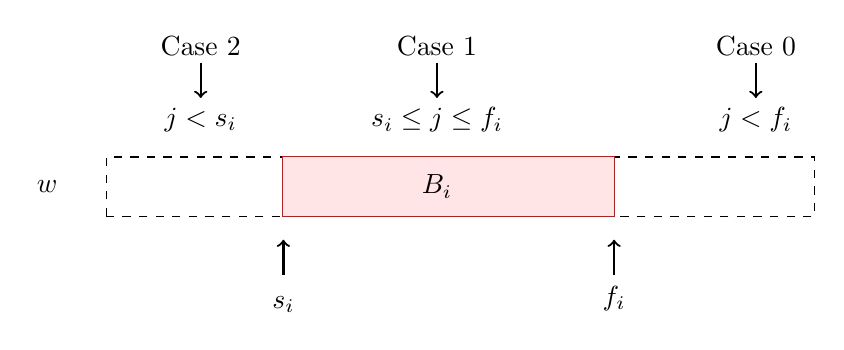
\begin{tikzpicture}[scale=1.5]
        % Main Rectangle w
        \draw[dashed] (0,0) rectangle (6,0.5);
        \node at (-0.5, 0.25) {\(w\)};

        % Smaller Rectangle 1 - Border color red
        \draw[draw=red, thick] (1.5,0) rectangle (4.3,0.5);
        
        \draw[->, thick] (1.5,-0.5) -- (1.5,-0.2);
        \node[align=center, below] at (1.5,-0.6) {\(s_{i}\)};
        \fill[red!10] (1.5,0) rectangle (4.3,0.5);
        \node at (2.8,0.25) {$B_{i}$};
        
        \draw[->, thick] (4.3,-0.5) -- (4.3,-0.2);
        
        \node at (4.3,-0.7) {$f_i$};
        
        
        \draw[->, thick] (5.5,1.3) -- (5.5,1);        
        \node[align=center, below] at (5.5,1) {\( j<f_i\)};
        \node[align=center, below] at (5.5,1.6) { \text{Case 0}};

        \draw[->, thick] (2.8,1.3) -- (2.8,1);        
        \node[align=center, below] at (2.8,1) {\( s_i \leq j \leq f_i\)};
        \node[align=center, below] at (2.8,1.6) {\text{Case 1}};

        \draw[->, thick] (0.8,1.3) -- (0.8,1);        
        \node[align=center, below] at (0.8,1) {\( j<s_i\)};
        \node[align=center, below] at (0.8,1.6) {\text{Case 2}};
        


    \end{tikzpicture}
    \caption{Compression for $w$ where $j$ is located.}
    \label{fig:case0}
\end{figure}


% So then, for case 0 $f_i<j$, it means that $s_i=s'_i$ and $f_i=f'_i$, LZ77 algorithm produces the exactly same result for $w[1,...,f_i]=w'[1,...,f_i]$, therefore. $B'_i$ is the only block that starts inside $B_i$, indeed, furthermore, $B_k=B'_k \forall k \leq i$.
% conclude that $f_i'\geq j$. When the case 1 holds, If $s_i\leq j\leq f_i$. We firstly have when $s_i=s'_i$, so that $B_k=B'_k \forall k \leq i-1$, this implies that $f_{i-1}=f'_{i-1}$. Hence $s_i=f_{i-1}+1 = f'_{i-1}+1 = s'_i$. We secondly have $f'_i\geq j$, so then, LZ77 compression only changes when a character is unknown for the string, thus, compression for $w'$ in the block $B'_i$ ends when $f_i=j$, moreover could be even greater, we never can finish before the index $j$ since compression up to $j$ is the same, so $|\mathcal{M}_i|= 1$ or $|\mathcal{M}_i|= 2$. Moreover, when $f'_{i+1}\geq f_i$, since $f_i\geq j$ we basically know that $f_i>f'_{i+1}$ but it does not matter how further $f'_{i+1}$ goes, because LZ77 compression guarantees that we can copy a substring that are previously encode. this automatically means that $|\mathcal{M}_i|= 2$ that is our important fact. On the other hand, analysis for case 2 relies when $j<s_i$ but based on LZ77 compression, when $j$ is placed before where the string for the block is copied over, it means that any place is located at compression for $w'$ adds at least 1 more block $B'_t$ that starts inside $B_k$ however since the condition holds we know that $f_i>f'_{i+1}$ therefore $|\mathcal{M}_i| \leq 2$.
% \end{proof}

% %%%%%%%%%%%%%%%%%%%%%%

% Let $t$ the maximum number of blocks after compressing $w'$ that \emph{Start Inside} $w$, since $w \sim w'$, then there is always a compression $(B'_1,...,B'_t)$ such as, WLOG $t'\geq t$ therefore, we defined $t'= \sum_{i=1}^{\infty}|\mathcal{M}_i|$, and $t= \sum_{i=1}^{\infty}|\mathcal{M}_i|$. These calculations are required for determine the quantity of blocks that \emph{Start Inside} either $B$ or $B'$ as a quantified property. Based on this reasoning and \defref{def:local_sensitivity} we introduce the difference to obtain Global Sensitivity, so then formally \claimref{claim:set:blocksm2:GS} as:
% %%%%%%%%%%%%%%%%%%%%%%%






% \lemblocknumupperbound

% \begin{proof}
%         If $i\in\B_2$ then either (1) $s_i\leq j\leq f_i$ or (2) $j-\ell_i < q_i \leq j$. When $j >f_i$, by LZ77 compression $B_i=B'_i$, thus $|\mathcal{M}_i|= 1$ and $i \in \mathcal{B_1}$.Hence, we have $s_i\leq j\leq f_i$ if $j\geq s_i$.
    
%     On the other hand, If $j<s_i$, then we want to show that $j-\ell_i<q_i\leq j$, i.e., $q_i\leq j < q_i+\ell_i$.
%     % \input{../Manuscript/figures/fig:claim9:case2}
%     Suppose for contradiction that $j\not\in[q_i,q_i+\ell_i-1]$.
%     Let $k$ be the smallest element in $\M_i$, i.e., $s_i\leq s_k'\leq f_i$ but $s_{k-1}'<s_i$.         
%     If $s_k'=f_i$, then if there is another $k'\in\M_i$ with $k'\neq k$, then by choice of $k$, we have $k<k'$ and therefore $s_{k'}'>f_k'>s_k'=f_i$. Hence, $|\M_i|= 1$ and $i\in\B_1$. Contradiction! It happens with any case for $j\not\in[q_i,q_i+\ell_i-1]$, since $i \in \B_2$. 
    
%     Now based on this, we are sure If $i_1,i_2\in\B_2$ then $(q_{i_1},\ell_{i_1})\neq(q_{i_2},\ell_{i_2})$. Since $i_1<i_2$ we then have $j<s_{i_1}<s_{i_2}$. Let $B_{i_1}=[q_{i_1},\ell_{i_1},c_{i_1}]$ and $B_{i_2}=[q_{i_2},\ell_{i_2},c_{i_2}]$ be  the blocks $B_{i_1}$ and $B_{i_2}$ of the LZ77 compression function $\compress:(\Sigma)^*\rightarrow(\Sigma')^*$ (Resp. w'). By intuition we know that there is no possibility to start in the same point for both Blocks $B_{i_1}$ and $B'_k$ after being read $j$ previously.
    

%     Finally Let $\B_2^\ell\coloneqq\{i\in\B_2:\ell_i=\ell\}$ and suppose that $s_{i^*}\leq j\leq f_{i^*}$ for some $i^*\in[t]$. Then $|\B_2^\ell|\leq\ell$ for all $\ell\neq \ell_{i^*}$, and $|\B_2^{\ell_{i^*}}|\leq\ell_{i^*}+1$. Furthermore, we observe that the constraint about length is: $\sum_{i\in\B_2} (\ell_i+1)\leq n,$ and $    \sum_\ell x_\ell'(\ell+1) < \sum_\ell x_\ell  (\ell+1) \leq n$. To find the threshold $z$, we observe that
% $\sum_{\ell=0}^z \ell(\ell+1) = \frac{1}{3}z(z+1)(z+2)\leq n,$
% which implies $z^3\leq 3n$ and $z\leq\sqrt[3]{3n}$. Setting this value of $z$, we have $t_2 \leq \frac{\sqrt[3]{9}}{2} n^{2/3} + \frac{\sqrt[3]{9}}{2} n^{1/3} + 1,$.
% \end{proof}

% The main result of this subsection is based on the analysis for upper bounding the global sensitivity, so then, in \secref{sec:upperbound} the goal is to provide the exact coefficient for the bound as is shown in the following theorem:




\section{Lower Bound for the Global Sensitivity of LZ77 Compression}\seclab{sec:lowerbound}

% =====

% \paragraph*{String Construction for the GS Lower Bound.}

% To prove the lower bound $\Omega(n^{2/3}\log^{1/3}n)$ for the global sensitivity of the LZ77 compression, we need to give example strings $w\sim w'$ of length $n$ that achieves $\left||\compress(w)|-|\compress(w')|\right|=\Omega(n^{2/3}\log^{1/3} n)$ (where $\compress$ denotes the LZ77 compression function) since this implies
% \begin{align*}
%     \mathtt{GS}_{\mathtt{Compress}} &= \max_{x \in \Sigma^n} \mathtt{LS}_{\mathtt{Compress}}(x)\\
%     &= \max_{x \in \Sigma^n}\max_{x' \in \Sigma^n:x\sim x'} \left| |\compress(x)| - |\compress(x')| \right|\\
%     &\geq \left||\compress(w)|-|\compress(w')|\right|\\
%     &=\Omega(n^{2/3}\log^{1/3} n).
% \end{align*}
% We give strings $w\sim w'$ that are carefully crafted such that $|w|=|w'|=\Theta(m^3\log m)$ for some integer $m>0$ and the number of type-2 blocks is $\Theta(m^2)$, which implies that $\GS_\compress=\Omega(m^2\log m) = \Omega(n^{2/3}\log^{1/3}n)$ where $n=\Theta(m^3\log m)$ denotes the length of strings. A core component of the string construction is to consider an \emph{injective encoding} of the number set $[m]$, which takes $\lceil\log m\rceil$ bits for each encoding, to ensure that each encoding is unique. This helps us count the number of type-2 blocks. However, having an injective encoding only does not fully resolve the issue 

% We overcome this bottleneck by \emph{repeating} each encoding twice.

% =====

In \secref{sec:upperbound}, we proved that the upper bound for the global sensitivity of the LZ77 compression algorithm $\compress$ is $O(n^{2/3}\log n)$ with window size $W=n$. One could ask if this is a tight bound, i.e., if we can prove the matching \emph{lower bound} for the global sensitivity of $\compress$ as well. This section proves the almost-matching lower bound up to a sub-logarithmic factor. In particular, we show that the global sensitivity of the LZ77 compression algorithm is $\Omega(n^{2/3}\log^{1/3} n)$. To prove the lower bound, we need to give example strings $w\sim w'$ of length $n$ that achieves $\left||\compress(w)|-|\compress(w')|\right|=\Omega(n^{2/3}\log^{1/3} n)$ since this implies $\GS_\compress=\max_{x \in \Sigma^n}\max_{x' \in \Sigma^n:x\sim x'} \left| |\compress(x)| - |\compress(x')| \right|\geq \left||\compress(w)|-|\compress(w')|\right|=\Omega(n^{2/3}\log^{1/3} n)$. 
% \begin{align*}
%     \mathtt{GS}_{\mathtt{Compress}} &= \max_{x \in \Sigma^n}\max_{x' \in \Sigma^n:x\sim x'} \left| |\compress(x)| - |\compress(x')| \right|\\
%     &\geq \left||\compress(w)|-|\compress(w')|\right|=\Omega(n^{2/3}\log^{1/3} n).
% \end{align*}
For the rest of \secref{sec:lowerbound}, we will give the construction of such example strings $w$ and $w'$.

\subsection{String Construction}

Consider an encoding function $\Enc:\mathbb{Z}\rightarrow\bin^*$ that maps integers to binary strings. Then for a positive integer $m\in\mathbb{Z}$, we have an injective encoding of the number set $\mathcal{S}\coloneqq\left\{0,1,\ldots, m\right\}$ using $\lceil\log m\rceil$ bits, i.e., $\Enc(i)\neq\Enc(j)$ if $i,j\in\mathcal{S}$ and $i\neq j$. For example, if $m=2^q-1$ for some positive integer $q$, we could encode the elements of $\S$ as follows: 
\[\Enc(0)=0^{\lceil\log m\rceil},\Enc(1)=0^{\lceil\log m\rceil-1}1,\Enc(2)=0^{\lceil\log m\rceil-2}10,\ldots,\Enc(m)=1^{\lceil\log m\rceil}.\] 
Now, consider a quinary alphabet $\Sigma=\{0,1,2,3,4\}$ and define a string
\[S_{\ell,u}\coloneqq\Enc(m-u+1)^2\circ\Enc(m-u+2)^2\circ\cdots\circ\Enc(m)^2\circ 2 \circ\Enc(m+1)^2\circ\cdots\circ\Enc(m-u+\ell)^2 \]
in $\Sigma^*$ for $2\leq\ell\leq m$ and $1\leq u\leq\ell-1$. 
Here, $(\cdot)^2$ denotes the concatenation of the string itself twice, i.e., $\Enc(\cdot)^2=\Enc(\cdot)\circ\Enc(\cdot)$. 
We define a procedure called $\QuinStr(m)$ which takes as input a positive integer $m\in\mathbb{Z}$ and outputs two quinary strings as follows.

\begin{tcolorbox}[breakable,enhanced,title={The Construction of Two Quinary Strings $\QuinStr(m)$.}]
    \begin{enumerate}
        \item The algorithm computes two quinary strings $S_w$ and $S_{w'}$ where
        \begin{align*}
            S_w &\coloneqq\Enc(1)^2\circ\cdots\circ\Enc(m)^2\circ 2 \circ\Enc(m+1)^2\circ\cdots\circ\Enc(2m)^2\circ 4,\text{ and}\\
            S_{w'} &\coloneqq\Enc(1)^2\circ\cdots\circ\Enc(m)^2\circ 3 \circ\Enc(m+1)^2\circ\cdots\circ\Enc(2m)^2\circ 4.
        \end{align*}
        \item Then it computes two quinary strings $w,w'$ defined as $w\coloneqq S_w\circ S$ and $w'\coloneqq S_{w'}\circ S$, where
        \[S = S_{2,1} \circ 4 \circ S_{3,2} \circ 4 \circ S_{3,1} \circ 4 \circ \ldots \circ S_{m,m-1} \circ 4 \circ \ldots \circ S_{m,1}\circ 4.\]
        \item Output $(w,w')$.
    \end{enumerate}
\end{tcolorbox}

\claimref{claim:length} tells us that the strings $w$ and $w'$ outputted by the procedure $\QuinStr(m)$ has equal length $\Theta(m^3\log m)$. Since the proof is elementary, we defer the proof of \claimref{claim:length} to \appref{app:missingprooflowerbound}.

\newcommand{\claimlength}{
Let $m\in\mathbb{N}$ and $(w,w')\gets\QuinStr(m)$. Then $|w|=|w'|=\Theta(m^3\log m)$. In particular, for $m\geq 4$, $\frac{2}{3}m^3\lceil\log m\rceil< |w|=|w'|< m^3\lceil\log m\rceil$.
}
\begin{claim}\claimlab{claim:length}
\claimlength
\end{claim}

\subsection{Analyzing the Sensitivity of $\QuinStr(m)$}

A central step in our sensitivity analysis for $\QuinStr(m)$ is precisely counting the type-2 blocks produced by the LZ77 compression scheme, as we observed in \secref{sec:upperbound}. \lemref{lem:gs} shows that for $(w,w')\gets\QuinStr(m)$, we have $|\B_2|=\frac{(m-1)m}{2}-(\lfloor\frac{m}{2}\rfloor-1)$. Intuitively, we first show that for $w=S_w\circ S$, there is no type-2 block for the blocks compressing $S_w$. Then the main insight is that we carefully crafted strings $w$ and $w'$ such that the marker symbol `4' becomes the endpoint for each block in $\compress(w)$ for the tail part $S$ of $w=S_w\circ S$. By repeating each encoding twice, we can ensure that most of the occurrences of $S_{\ell,u}\circ 4$ yield type-2 blocks, with an edge case (addressed in \claimref{claim:repeat}) that makes the block in $\B_1$ but this happens for only about $m/2$ blocks. Consequently, despite these few exceptions, the overall count of type-2 blocks remains quadratic in $m$.

\newcommand{\lemGS}{
Let $m\in\mathbb{N}$ and $(w,w')\gets\QuinStr(m)$ and let $\compress:\Sigma^*\rightarrow(\Sigma')^*$ be the LZ77 compression algorithm. Let $(B_1,\ldots,B_t)\gets\compress(w)$ and $(B'_1,\ldots,B'_{t'})\gets\compress(w')$. Then $|\B_0| = 0$ and $|\B_2| = \frac{(m-1)m}{2}-(\lfloor\frac{m}{2}\rfloor-1)$.
}
\begin{lemma}\lemlab{lem:gs}
    \lemGS
\end{lemma}

\begin{proof}
Recall that $w = S_w \circ S$ and $w' = S_{w'} \circ S$, where
\begin{itemize}
    \item $S_w =\Enc(1)^2\circ\cdots\circ\Enc(m)^2\circ 2 \circ\Enc(m+1)^2\circ\cdots\circ\Enc(2m)^2\circ 4$,
    \item $S_{w'}=\Enc(1)^2\circ\cdots\circ\Enc(m)^2\circ 3 \circ\Enc(m+1)^2\circ\cdots\circ\Enc(2m)^2\circ 4$, and
    \item $S=S_{2,1} \circ 4 \circ S_{3,2} \circ 4 \circ S_{3,1} \circ 4 \circ \ldots \circ S_{m,m-1} \circ 4 \circ \ldots \circ S_{m,1}\circ 4$, where
    \item $S_{\ell,u}\coloneqq\Enc(m-u+1)^2\circ\Enc(m-u+2)^2\circ\cdots\circ\Enc(m)^2\circ 2 \circ\Enc(m+1)^2\circ\cdots\circ\Enc(m-u+\ell)^2$ for $2\leq\ell\leq m$ and $1\leq u\leq \ell-1$.
\end{itemize}
We first observe that $w\sim w'$. Define $S_w^F\coloneqq \Enc(1)^2\circ\cdots\circ\Enc(m)^2\circ 2$ (resp. $S_{w'}^F\coloneqq \Enc(1)^2\circ\cdots\circ\Enc(m)^2\circ 3$) to be the first-half substring of $S_w$ (resp. of $S_{w'}$), and $S_w^L=S_{w'}^L\coloneqq \Enc(m+1)^2\circ\cdots\circ\Enc(2m)^2\circ 4$ to be the last-half substring of $S_w$ (or $S_{w'}$ since they are indeed identical). 
It is useful to define a notation $\str(B_k)$ for a block $B_k$, which denotes the substring of $w$ represented by the block $B_k$, i.e., for $B_k=[q_k,\ell_k,c_k]$, $\str(B_k)\coloneqq w[q_k,q_k+\ell_k-1]\circ c_k$. 

Let $B_{i_1}$ be the first block such that $S_w^F$ becomes a substring of $\str(B_1)\circ\str(B_2)\circ\ldots\circ\str(B_{i_1})$, and similarly, let $B'_{i'_1}$ be the first block such that $S_{w'}^F$ becomes a substring of $\str(B'_1)\circ\str(B'_2)\circ\ldots\circ\str(B'_{i'_1})$. Then we observe the following:
\begin{enumerate}
    \item $B_{i_1}=[q_{i_1},\ell_{i_1},2]$, i.e., $\str(B_{i_1})$ ends with $2$ (which is the last character in $S_w^F$), since $2$ never showed up before as all the encodings are binary strings, it has to be added to the dictionary as a new character,
    \item $B_i=B_i'$ for all $i\in[i_1-1]$, as we are compressing the identical strings until we see $2$ in $S_w^F$ (and $3$ in $S_{w'}^F$), and
    \item $i_1=i_1'$ and $B'_{i_1}=[q_{i_1},\ell_{i_1},3]$, since two strings $S_w^F$ and $S_{w'}^F$ are identical except for the very last character.\label{item:2}
\end{enumerate}

Now let $B_{i_2}$ be the first block such that $S_w^L$ becomes a substring of $\str(B_{i_1+1})\circ\str(B_{i_1+2})\circ\ldots\circ\str(B_{i_2})$, and similarly, let $B'_{i'_2}$ be the first block such that $S_{w'}^L$ becomes a substring of $\str(B'_{i_1+1})\circ\str(B'_{i_1+2})\circ\ldots\circ\str(B'_{i'_2})$. Then we observe the following:
\begin{enumerate}
\setcounter{enumi}{3}
    \item $i_2=i_2'$ and $B_i=B_i'$ for all $i\in[i_1+1,i_2]$, since $i_1=i_1'$ from observation \ref{item:2} and we have $S_w^L=S_{w'}^L$ while they do not contain $2$ or $3$, and
    \item $B_{i_2}=[q_{i_2},\ell_{i_2},4]$, since $4$ never showed up before in our compression.
\end{enumerate}

From the observations above, we have that $B_i\in\B_1$ for all $i\in[i_2]$. 
Now we are left with the blocks $(B_{i_2+1},\ldots,B_t)$ compressing the last part $S$ of $w$ and the blocks $(B'_{i_2+1},\ldots,B'_{t'})$ compressing the last part $S$ of $w'$. For the blocks $(B_{i_2+1},\ldots,B_t)$, we observe that each block ends at the next `$4$' because each $S_{\ell,u}$ (for $2\leq\ell\leq m$ and $1\leq u\leq \ell-1$) is contained in the former part of $w$ (which was $S_w$) but $4$ only shows up in $S_w$ followed by $\Enc(2m)^2$ while $S_{\ell,u}$ cannot contain $\Enc(2m)$. Hence, we observe the following:
\begin{enumerate}
\setcounter{enumi}{5}
    \item $\str(B_{i_2+1})=S_{2,1}\circ 4,\str(B_{i_2+2})=S_{3,2}\circ 4$,  and so on.
    \item In general, $\str\left(B_{i_2+\frac{(\ell-2)(\ell-1)}{2}+(\ell-t)}\right)=S_{\ell,u}\circ 4$, for $2\leq\ell\leq m$ and $1\leq u\leq \ell-1$. This indeed covers all the blocks from $B_{i_2+1},\ldots,B_t$ (See \claimref{claim:inj} and observation \ref{item:8}).
    \item Furthermore, we can observe that $t= i_2 + (1+2+\ldots+(m-1)) = i_2 + \frac{(m-1)m}{2}$.\label{item:8}
\end{enumerate}

\newcommand{\felluinjective}{
For any integer $m\geq 2$, the function $f(\ell,u)\coloneqq\frac{(\ell-2)(\ell-1)}{2}+(\ell-u)$ defined over integers $\ell$ and $u$ such that $2\leq \ell\leq m$ and $1\leq u\leq \ell-1$ is injective, and its range is $[\frac{(m-1)m}{2}]$.
}
\begin{claim}\claimlab{claim:inj}
\felluinjective
\end{claim}

The proof of \claimref{claim:inj} is elementary by induction on $m$, and hence, we defer the proof to \appref{app:missingprooflowerbound}. What we are interested in is whether each $B_i$, for $i_2+1\leq i\leq t$, belongs to $\B_0$, $\B_1$, or $\B_2$. In \claimref{claim:blocks}, we prove that the blocks are mostly in $\B_2$ and the rest of the blocks are in $\B_1$, meaning that $\B_0=\emptyset$. In particular, we prove that for $2\leq\ell\leq m$ and $1\leq u\leq\ell-1$, $B_{i_2+\frac{(\ell-2)(\ell-1)}{2}+(\ell-u)}\in\B_1$ if and only if all of these conditions hold: (1) $\ell>2$, (2) $\ell$ is even, and (3) $u=\ell/2$. 

\begin{claim}\claimlab{claim:blocks}
For $2\leq\ell\leq m$ and $1\leq u\leq \ell-1$, $B_{i_2+\frac{(\ell-2)(\ell-1)}{2}+(\ell-u)}\in\B_1$ if and only if $\ell>2, 2\mid\ell$, and $u=\ell/2$; otherwise $B_{i_2+\frac{(\ell-2)(\ell-1)}{2}+(\ell-u)}\in\B_2$.
%For $\ell'\in\left[\lfloor\frac{m}{2}\rfloor\right]$, $B_{i_2+(\ell'-1)(2\ell'-1)+\ell'}\in\B_1$ and 
\end{claim}

We will give the proof of \claimref{claim:blocks} below and finish the proof of \lemref{lem:gs} first for readability. By \claimref{claim:blocks}, since there are only $\lfloor\frac{m}{2}\rfloor-1$ of such pairs of $(\ell,u)$, we observe that $|\B_2|=\frac{(m-1)m}{2}-(\lfloor\frac{m}{2}\rfloor-1)$. Since we have that $B_i\in\B_1$ for all $i\in[i_2]$, we have $\B_0=\emptyset$ and therefore $|\B_0|=0$. This completes the proof of \lemref{lem:gs}.
\end{proof}

\begin{proofof}{\claimref{claim:blocks}}
Recall that $S=S_{2,1}\circ4\circ S_{3,2}\circ4\circ S_{3,1}\circ4\circ\ldots\circ S_{m,m-1}\circ4\circ\ldots\circ S_{m,1}\circ4$ and $\str(B_{i_2+1})=S_{2,1}\circ4$, $\str(B_{i_2+2})=S_{3,2}\circ4$, $\str(B_{i_2+3})=S_{3,1}\circ4,\ldots,\str(B_t)=S_{m,1}\circ4$. 
For each $S_{\ell,u}$, we observe that $S_{\ell,u}$ is \emph{not} a substring of $S_{w'}$. Hence, we see that each block $B_i$ (for $i_2+1\leq i\leq t$) is roughly split into two blocks for the blocks of $\compress(w')$ unless it could copy beyond the character $4$. To observe the cases when this happens,
for each $S_{\ell,u}$, it is helpful to define:
\begin{itemize}
    \item $S_{\ell,u}^F\coloneqq\Enc(m-u+1)^2$ denotes the very first encoding concatenation that shows in $S_{\ell,u}$, 
    \item $S_{\ell,u}^{F,(1/2)}\coloneqq\Enc(m-u+1)$ denotes the very first encoding in $S_{\ell,u}$ (i.e., half of $S_{\ell,u}^F$),
    \item $S_{\ell,u}^L\coloneqq\Enc(m-u+\ell)^2$ denotes the very last encoding concatenation that shows in $S_{\ell,u}$, and
    \item For $k>u$, $S_{\ell,u}^{(k)}\coloneqq\Enc(m-u+1)^2\circ\Enc(m-u+2)^2\circ\ldots\circ\Enc(m)^2\circ2\circ\Enc(m+1)^2\circ\ldots\circ\Enc(m-u+k)^2$ denotes the first $k$ encoding concatenations that shows in $S_{\ell,u}$.
\end{itemize}
Then we observe the following claims. Since proofs of \claimref{claim:notrepeat} and \claimref{claim:repeat} are elementary, we defer the proofs to \appref{app:missingprooflowerbound}.

\begin{claim}\claimlab{claim:notrepeat}
$S_{\ell,u}^L\circ4\circ S_{\ell,u-1}^F$ does not repeat for different $\ell$ and $u$ such that $3\leq\ell\leq m$ and $2\leq u\leq\ell-1$.
\end{claim}

\claimref{claim:notrepeat} tells us that, due to the injectivity of the encoding, any block in $\compress(w')$ containing a portion of $S_{\ell,u}^L$ along with the delimiter `4' must finish at $S_{\ell,u}^{F,(1/2)}$ in the worst case. In particular, note that $S_{\ell,u}^L=\Enc(m-u+\ell)^2=S_{\ell+1,u+1}^L$ for $3\leq \ell<m$ and $2\leq u<\ell-1$. Moreover, we have $S_{\ell,u-1}^{F,(1/2)}=\Enc(m-u+2)$ and $S_{\ell+1,u}^{F,(1/2)}=\Enc(m-u+1)$, which can agree on all but the final bit (e.g., $S_{\ell,u-1}^{F,(1/2)}=00\cdots00$ and $S_{\ell+1,u}^{F,(1/2)}=00\cdots01$). Without the repetition of each encoding, a block might incorporate nearly the entire $S_{\ell+1,u}^{F,(1/2)}$ except for the last bit. Consequently, by having this last bit as a new character, $S_{\ell,u-1}\circ4$ would be placed in $\B_1$. Repeating the encoding twice eliminates this possibility and we can ensure that the scenario described in \claimref{claim:repeat} is the only case where type-1 blocks would occur. Again, see \appref{app:missingprooflowerbound} for the proof of \claimref{claim:repeat}.


\begin{claim}\claimlab{claim:repeat}
For $2\leq\ell\leq\lfloor\frac{m}{2}\rfloor-1$, $S_{\ell,1}^L\circ4\circ S_{\ell+1,\ell}$ repeats at $S_{2\ell,\ell+1}^L\circ4\circ S_{2\ell,\ell}^{(\ell+1)}$.
\end{claim}

Let's go back to the proof of \claimref{claim:blocks}. By \claimref{claim:repeat}, we can see that the block of the form $B_{i_2+\frac{(2\ell-2)(2\ell-1)}{2}+(2\ell-\ell)}$ which satisfies
\[\str\left(B_{i_2+\frac{(2\ell-2)(2\ell-1)}{2}+(2\ell-\ell)}\right)=S_{2\ell,\ell}\circ4,\]
is in $\B_1$, and all of the other blocks beyond $B_{i_2}$ are in $\B_2$. This completes the proof of \claimref{claim:blocks}.
% We first observe the following.
% Now, let's analyze the blocks $(B'_{i_2+1},\ldots,B'_{i'_3})$. Consider $B'_{i_2+1}$ first as a warmup. Recall that $\str(B_{i_2+1})=S_{2,1}\circ 4$ because $S_{2,1}=\Enc(m)^2\circ 2\circ \Enc(m+1)^2$ was a substring of $S_w$, but this is \emph{not} the case for $w'$ since we replaced $2$ with $3$ in $S_{w'}$. This observation implies that $\str(B'_{i_2+1})=\Enc(m)^2\circ 2$ (which is the substring of $S_{2,1}$) since $\Enc(m)^2$ was contained in $S_{w'}$ and it is indeed the longest substring you could copy from the prior substring since $2$ never showed up in $w'$.
% Next, consider the next block $B'_{i_2+2}$. It is easy to see that $\str(B'_{i_2+2})=\Enc(m+1)^2\circ 4$ because $\Enc(m+1)^2$ is a substring of $S_{w'}$ and $4$ only showed up once in a prior substring, followed by $\Enc(2m)^2$ (in $S_{w'}\circ 4$). With a similar argument, we observe that $\str(B'_{i_2+3})=\Enc(m-1)^2\circ\Enc(m)^2\circ 2$ (which is a substring of $S_{3,2}$). Now for the block $B'_{i_2+4}$, one might think that $\str(B'_{i_2+4})=\Enc(m+1)^2\circ 4\circ c'_{i_2+4}$ where $c'_{i_2+4}$ is the first character in $\Enc(m)$ (since $S_{3,1}$ starts with $\Enc(m)^2$) since it seems to be the case that $\Enc(m+1)^2\circ 4$ is the longest substring of $S_{w'}\circ 4 \circ S_{2,1}\circ 4\circ \Enc(m-1)^2\circ\Enc(m)^2\circ 2$
\end{proofof}

Taken altogether, we can lower bound the global sensitivity of the LZ77 compression scheme as stated in \thmref{thm:lowerbound} below.

\begin{theorem}\thmlab{thm:lowerbound}
Let $\compress:\Sigma^*\rightarrow\Sigma'^*$ be the LZ77 compression function. Then $\mathtt{GS}_\compress\geq 4^{-1/3}\cdot n^{2/3}\log^{1/3}n=\Omega(n^{2/3}\log^{1/3}n)$. 
\end{theorem}

\begin{proof}
Let $(w,w')\gets\QuinStr(m)$ and let $|w|=|w'|=n$. By \claimref{claim:length}, we have $|w|=|w'|=\Theta(m^3\log m)$ and therefore $n=\Theta(m^3\log m)$. Furthermore, \claimref{claim:length} tells us that there exists some $\alpha$ with $\frac{2}{3}\leq\alpha\leq 1$ such that $n=\alpha m^3\log m$.  
Now let $(B_1,\ldots,B_t)\gets\compress(w)$ and $(B'_1,\ldots,B'_{t'})\gets\compress(w')$.
Recall that if we look at the proof of \claimref{claim:set:blocksm2:GS}, it tells us that $t'-t=|\B_2|-|\B_0|$. From \lemref{lem:gs}, we have $|\B_0|=0$ and $|\B_2|=\frac{(m-1)m}{2}-(\lfloor\frac{m}{2}\rfloor-1)$, which implies that $t'-t=\frac{(m-1)m}{2}-(\lfloor\frac{m}{2}\rfloor-1)$. We know $|\compress(w)|=t(2\lceil\log n\rceil+\lceil\log|\Sigma|\rceil)$ and $|\compress(w')|=t'(2\lceil\log n\rceil+\lceil\log|\Sigma|\rceil)$, we have
\begin{align*}
   \mathtt{GS}_{\mathtt{Compress}} & \leq  \left||\compress(w)|-|\compress(w')|\right|  
   = |t-t'|\left(2\lceil\log n\rceil+\lceil\log|\Sigma|\rceil\right) \\
    &= |t-t'|\left(2\left\lceil\log (\alpha m^3\log m)\right\rceil+\lceil\log|\Sigma|\rceil\right) 
    %\geq \left[\frac{(m-1)m}{2}-\left(\left\lfloor\frac{m}{2}\right\rfloor-1\right)\right]\cdot2\log(\alpha m^3\log m)\\
    \geq \frac{m^2}{4}\cdot 4\log m = m^2\log m \ .
\end{align*}
% \begin{align*} backup for full version
%     \left||\compress(w)|-|\compress(w')|\right| &= |t-t'|\left(2\lceil\log n\rceil+\lceil\log|\Sigma|\rceil\right) \\
%     &= |t-t'|\left(2\left\lceil\log (\alpha m^3\log m)\right\rceil+\lceil\log|\Sigma|\rceil\right)\\
%     &\geq \left[\frac{(m-1)m}{2}-\left(\left\lfloor\frac{m}{2}\right\rfloor-1\right)\right]\cdot2\log(\alpha m^3\log m)\\
%     &\geq \left(\frac{m^2}{2}-m\right)\cdot 4\log m\\
%     &\geq \frac{m^2}{4}\cdot 4\log m = m^2\log m,
% \end{align*}
%which implies that
%\begin{align*}
 %   \mathtt{GS}_{\mathtt{Compress}} &= \max_{x \in \Sigma^n}\max_{x' \in \Sigma^n:x\sim x'} \left| |\compress(x)| - |\compress(x')| \right|\\
 %   &\geq \left||\compress(w)|-|\compress(w')|\right|\\
  %  &= m^2\log m.
%\end{align*}
Furthermore, since we have $n=\alpha m^3\log m$ for some $\frac{2}{3}\leq\alpha\leq 1$, we observe that
\begin{align*}
    m^2\log m &= m^2\cdot\frac{n}{\alpha m^3}= \frac{n}{\alpha}\cdot\frac{1}{m} = \frac{n}{\alpha}\cdot\frac{\alpha^{1/3}\cdot\log^{1/3}m}{n^{1/3}}
    \geq \left(\frac{n}{\alpha}\right)^{2/3}\cdot 4^{-1/3}\cdot\log^{1/3}n \\
    &\geq 4^{-1/3}\cdot n^{2/3}\log^{1/3}n,
\end{align*}
% \begin{align*} backup for full version
%     m^2\log m &= m^2\cdot\frac{n}{\alpha m^3}\\
%     &= \frac{n}{\alpha}\cdot\frac{1}{m}\\
%     &= \frac{n}{\alpha}\cdot\frac{\alpha^{1/3}\cdot\log^{1/3}m}{n^{1/3}}\\
%     &= \left(\frac{n}{\alpha}\right)^{2/3}\cdot\log^{1/3}m\\
%     &\geq \left(\frac{n}{\alpha}\right)^{2/3}\cdot 4^{-1/3}\cdot\log^{1/3}n\\
%     &\geq 4^{-1/3}\cdot n^{2/3}\log^{1/3}n,
% \end{align*}
where the first inequality comes from the observation $\log n = \log\alpha + 3\log m + \log\log m\leq 4\log m$ and the second inequality comes from $(1/\alpha)\geq 1$. Hence,
\begin{align*}
    \mathtt{GS}_{\mathtt{Compress}} &\geq m^2\log m \geq 4^{-1/3}\cdot n^{2/3}\log^{1/3}n,
\end{align*}
% Since we know $\frac{2}{3}\cdot m^3\log m\leq n\leq m^3\log m$ from \claimref{claim:length}, we observe that 
% \begin{align*}
%     m^2\log m &= \frac{1}{m}\cdot m^3\log m\\
%     &\geq \frac{1}{m}\cdot n\\
%     &\geq \sqrt[3]{\frac{2}{3}}\cdot n^{-1/3}\cdot\left(\log^{1/3}m\right)\cdot n\\
%     &\geq \sqrt[3]{\frac{2}{3}}\cdot n^{-1/3}\cdot\left(\sqrt[3]{\frac{1}{6}}\cdot\log^{1/3}n\right)\cdot n\\
%     &= \sqrt[3]{\frac{1}{9}}\cdot n^{2/3}\log^{1/3}n,
% \end{align*}
% where the third inequality is achieved by the observation that $3\log m\geq \log n - \log\log m \geq \frac{\log n}{2}$, since $\log m\leq \sqrt{n}$.
% Hence,
% \begin{align*}
%     \mathtt{GS}_{\mathtt{Compress}} &\geq m^2\log m\\
%     &\geq \sqrt[3]{\frac{1}{9}}\cdot n^{2/3}\log^{1/3}n,
% \end{align*}
which completes the proof.
\end{proof}
  \caption{Sensitivity Bar Plot.}
  \label{fig:CHOA-sensitivity}
  \end{subfigure}
  \hfill
  \begin{subfigure}[b]{0.245\textwidth}
  \centering
  \begin{tikzpicture}
    \begin{axis}[
        width=\linewidth,
        ylabel style={font=\scriptsize,yshift=-0.6em},
        y tick label style={font=\scriptsize},
        x tick label style={font=\scriptsize},
        ybar,
        %axis lines=left,  
        ymajorgrids,
        symbolic x coords={XGBoost, gMLP, PedCA-FT},
        %xtick={XGBoost, LightGBM, {ours}},
        ylabel={Specificity},
        ymin=0,
        ymax=110,
        bar shift=0pt,
        %bar width=0.5cm,
        nodes near coords, 
        nodes near coords style={font=\scriptsize}, 
        %enlargelimits=0.10,
    ]
        \addplot[
            fill=Set2-A,
            ybar,
            error bars/.cd,
            y dir=both,
            y explicit,
        ] coordinates {
            (XGBoost, 83.14) += (0, 1.06) -= (0, 1.12)
        };
        \addplot[
            fill=Set2-B,
            ybar,
            error bars/.cd,
            y dir=both,
            y explicit,
        ] coordinates {
            (gMLP, 97.0) += (0, 0.45) -= (0, 0.54)
        };
        \addplot[
            fill=Set2-C,
            ybar,
            error bars/.cd,
            y dir=both,
            y explicit,
        ] coordinates {
            (PedCA-FT, 84.69) += (0, 0.02) -= (0, 1.08)
        };
    \end{axis}
\end{tikzpicture}
  \caption{Specificity Bar Plot.}
  \label{fig:CHOA-specificity}
  \end{subfigure}
  \caption{Bar plots with error bars illustrating PPV, NPV, Sensitivity, and Specificity.}
  \label{fig:bar_chart}
\end{figure*}


\begin{figure*}
\centering
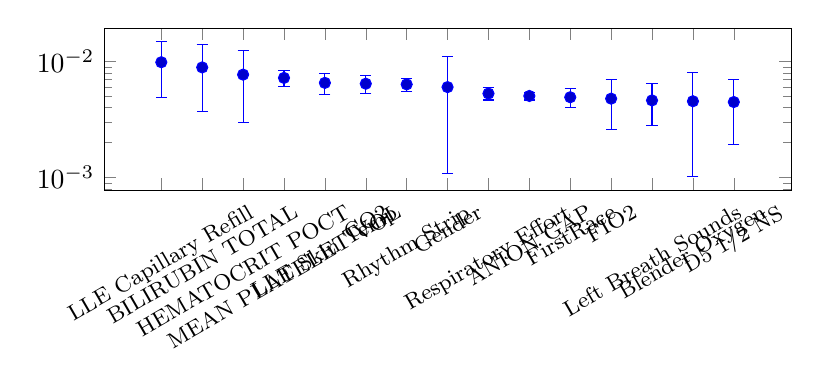
\begin{tikzpicture}
\begin{semilogyaxis} [
width=0.85\linewidth,
height=0.3\linewidth,
%log ticks with fixed point,
symbolic x coords={LLE Capillary Refill,BILIRUBIN TOTAL,HEMATOCRIT POCT,MEAN PLATELET VOL,LLE Skin Temp,CO2,Rhythm Strip,Gender,Respiratory Effort,ANION GAP,FirstRace,FIO2,Left Breath Sounds, Blender Oxygen,D5 1/2 NS},
xtick=data,
%ytick=data,
ymode=log, % Set y-axis to logarithmic scale
log basis y={10}, % Base 10 logarithm for the y-axis
xticklabel style = {font=\footnotesize, rotate=30},
]
\addplot+[only marks] plot[error bars/.cd, y dir=both, y explicit]
coordinates{
    (LLE Capillary Refill,0.00986033870379835) +- (0.0147661644336152,0.00495451297398151)
    (BILIRUBIN TOTAL,0.00889949693092115) +- (0.0126273414402402,0.00517165242160214) 
    (HEMATOCRIT POCT,0.00771484551610147) +- (0.0106733043693973,0.00475638666280566)
    (MEAN PLATELET VOL,0.00722791639121327) +- (0.0155413424057195,-0.00108550962329301)
    (LLE Skin Temp,0.00654834543779) +- (0.0117898135027299,0.00130687737285006)
    (CO2,0.00643982552509323) +- (0.0117188530496206,0.00116079800056584)
    (Rhythm Strip,0.0063570944708815) +- (0.0135076080519946,-0.00079341911023163)
    (Gender,0.0060215957123226) +- (0.007101505027428,0.00494168639721721)
    (Respiratory Effort,0.00529990635784179) +- (0.00995787056878017,0.000641942146903415)
    (ANION GAP,0.00505141865792101) +- (0.00971814564992059,0.000384691665921432)
    (FirstRace,0.00492530982150281) +- (0.00893863381241345,0.000911985830592171)
    (FIO2,0.00478955726231307) +- (0.00737036239483328,0.00220875212979286)
    (Left Breath Sounds,0.00462497034406318) +- (0.00745013982514881,0.00179980086297755)
    (Blender Oxygen,0.00454991688743892) +- (0.00556981498211942,0.00353001879275842)
    (D5 1/2 NS,0.00447869625451364) +- (0.00641773512494759,0.00253965738407969)
};
\end{semilogyaxis} 
\end{tikzpicture}
\caption{Feature importance analysis using feature permutation. Error bar indicates p95 high and p95 low.}
\label{fig:feat_important}
\vspace{-0.4cm}
\end{figure*}


\subsection{Experimental Results \& Discussion}
Table~\ref{tab:CHOA_main_exp} summarizes the performance of our proposed \modelname to ten baseline models on various evaluation metrics. 
Notably, \modelname achieves the highest Bal\_acc, F1, MCC, and AUPRC outperforming all baseline models by an average improvement of $10.71$, $9.45$, $9.55$, and $3.10$ separately. 
Additionally, \modelname ranks second in AUROC, with an average improvement of $11.57$ except for gMLP model. 
Among baseline models, XGBoost achieves the runner-up in Bal\_Acc, F1, and MCC, while gMLP achieves the second best in AUPRC and the highest AUROC. 
The slightly lower AUROC of \modelname compared to gMLP can be attributed to AUROC's emphasis on overall ranking separability, which does not necessarily translate into optimal classification decisions~\cite{tomavsev2021use}, particularly in highly imbalanced datasets. AUROC measures the ability of a model to distinguish between control and case classes across all possible classification thresholds. However, it averages performance across all thresholds and gives equal importance to the classification of both the majority (control) and minority (CA) classes. In highly imbalanced datasets such as the pediatric CA prediction scenario, this can be problematic because the model might perform well on predicting non-CA patients and still achieve a high AUROC, even if it struggles to correctly identify patients at high risk of CA. 
Furthermore, our results highlight the effectiveness of multimodal data fusion. Models based on tabular representations (i.e., those using last observed risk factors) generally achieve superior Bal\_Acc, F1, and MCC, whereas models leveraging time-series representations tend to perform better in AUPRC and AUROC. Integrating a tabular transformer to capture complex interactions among high-dimensional tabular risk factors and a pre-trained textual transformer to effectively model the dynamics of textualized time-series risk factors, \modelname delivers SOTA performance for CA risk prediction.

% bar chart
We further analyze XGBoost, gMLP, and \modelname in terms of Positive Predictive Value (PPV), Negative Predictive Value (NPV), Sensitivity, and Specificity, as shown in Figure~\ref{fig:bar_chart}, to align with clinical priorities. Overall, \modelname achieves the most balanced performance across all four metrics.
Specifically, \modelname demonstrates a slight advantage in both PPV and NPV, while gMLP exhibits high variance in PPV, as indicated by the wide error bars. Notably, \modelname attains the highest sensitivity, which is particularly crucial for screening CA, where missing cases can have severe consequences. At the same time, \modelname maintains competitive specificity, striking a careful balance between sensitivity and specificity—two metrics that often trade off inversely.
These observations further validate the limitations of AUROC as a sole evaluation metric, highlighting its tendency to be overly optimistic or misleading in highly imbalanced settings. While AUROC emphasizes ranking separability, it does not directly reflect clinical utility, whereas metrics like sensitivity and PPV better capture a model’s practical impact on early CA detection.


\subsection{Feature Importance Analysis}
We use permutation importance method~\cite{altmann2010permutation} to calculate the feature importance scores for our proposed perturbed copy of the data where this feature's values have been randomly shuffled across rows. We set number of different permutation shuffles as $5$, and the confidence level as $0.95$. Top 15 important features with $p\_value \leq 0.05$ are presented in Fig.~\ref{fig:feat_important}.
Our analysis reveals that key clinical indicators, such as capillary refill, total bilirubin level, and hematocrit, are among the most important predictors for pediatric cardiac arrest. 
Notably, factors related to hemodynamic stability and oxygenation/ventilation—including CO2 level on arterial blood gas, and FIO2,—also rank highly, emphasizing their critical role in patient monitoring. Furthermore, the inclusion of demographic factors such as sex and race highlights the multifactorial nature of cardiac arrest risk in the pediatric population.
Overall, this feature importance analysis not only identifies clinical risk factors but also uncovers novel predictors that may enhance early risk detection and guide future targeted interventions.

%\subsection{Ablation Study of Two Base Models}